\chapter{Implementazione}
\label{cap:implementazione}

\section{Breve descrizione del programma}
Per lo studio di quanto descritto fino ad ora si è costruito un programma in grado di caricare un file \lstinline{.wav} in buffer di dimensione arbitraria in memoria per poterne elaborare il contenuto; dopodiché è possibile specificare una catena di operazioni da effettuare sul segnale e un metodo di salvataggio del risultato (\lstinline{.wav} o \lstinline{.csv}). La catena di operazioni e il salvataggio vengono specificati in un file di testo. Per la lettura e scrittura su file .wav si utilizza la libreria ``libsndfile'' scritta da Erik de Castro Lopo \cite{libsndfile}.

L'invocazione del programma avviene tramite riga di comando ed è necessario utilizzare un programma esterno per visualizzare il contenuto dei file di output. I grafici dei risultati che verranno mostrati in questa tesi sono stati generati utilizzando un file \lstinline{.csv} in uscita dal programma il quale viene poi visualizzato tramite il programma Veusz \cite{veusz}.

\section{Strutture dati utilizzate}

Per la rappresentazione dei dati dei campioni in ingressi si utilizza una struttura nominata \lstinline{SignalBuffer_t} definita nel seguente modo:

\begin{lstlisting}
struct SignalBuffer_t
{
    cuComplex* samples;
    size_t size;
    size_t max_size;
};
\end{lstlisting}

Essa continene un array di campioni, la lunghezza corrente e la lunghezza massima dello stesso. Questa struttura dati viene utilizzata sia dalla CPU sia dalla GPU e l'utilizzo di un array è necessario perché CUDA, senza librerie aggiuntive esterne, non riesce a gestire nei kernel gli oggetti della libreria standard di template di C++, di cui fa parte il template \lstinline{vector}.

Vengono definite anche operazioni su questa struttura, le quali ne garantiscono la corretta creazione, eliminazione e la corrispettiva gestione dei campioni all'interno della stessa. Le funzioni utilizzate sono dichiarate con i modificatori \lstinline{__host__ __device__} i quali sono necessari per segnalare al compilatore \lstinline{nvcc} che tali funzioni possono essere sia eseguite sulla CPU (host), sia sulla scheda grafica (device).

Infine \lstinline{cuComplex} è un tipo importato dalla libreria di CUDA il quale rappresenta un numero complesso. Esso può essere utilizzato, con le apposite operazioni, sia dalla CPU sia dalla GPU.

\section{Convoluzione}
Il primo algoritmo che è stato studiato e implementato è la convoluzione tra segnali la quale è indispensabile perché è il primo strumento con cui si può calcolare la risposta di un sistema ad un determinato segnale, a patto che si conosca la risposta impulsiva del sistema stesso.

La definizione di convoluzione tra segnali discreti è descritta dall'equazione \ref{eq:convoluzionediscreta}. Bisogna porre particolare attenzione al fatto che la lunghezza del risultato della convoluzione è uguale alla somma delle lunghezze dei segnali in ingresso meno uno; ciò comporta che sia necessario gestire il fenomeno detto ``overlap'' tra buffer risultanti consecutivi; questo fenomeno, grazie alla linearità del sistema, si riduce solamente alla somma della ``coda'' del buffer in uscita precedente con i primi campioni del buffer in uscita seguente.

Visto che la convoluzione è un'operazione che necessita di due segnali in entrata, si è supposto che il secondo segnale non sia diviso in vari buffer, ma sia tutto contenuto in uno solo, mentre il primo segnale può essere diviso in più buffer. Questa decisione è giustificata dal fatto che spesso la convoluzione viene utilizzata tra un segnale molto lungo e uno di gran lunga più corto, poiché, come già detto, è una operazione onerosa in termini di calcolo. In particolare è spesso utilizzata per operazioni di filtraggio e in questo caso il secondo segnale prende il nome di ``kernel del filtro'' \cite[p.~108]{dspguide}.

Nelle spiegazioni seguenti si utilizzerà la parola ``kernel'' per indicare il secondo segnale della convoluzione; bisogna prestare attenzione a non confondere il ``kernel'' del filtro con le funzioni ``kernel'' di CUDA.

\subsection{CPU}

La convoluzione sulla CPU è implementata utilizzando due cicli \lstinline{for}: uno che scorre i campioni del buffer in entrata di un determinato canale e l'altro invece che scorre i campioni del buffer contenente il secondo segnale. I due campioni ottenuti vengono quindi moltiplicati assieme e vengono poi aggiunti al valore di un buffer temporaneo. La presenza del buffer temporaneo è necessaria per la corretta gestione del fenomeno dell'``overlap''; il buffer temporaneo alla fine della convoluzione conterrà i campioni in uscita dalla convoluzione e la ``coda'' da sommare alla convoluzione successiva.

Una versione semplificata alle componenti fondamentali del codice che è stato utilizzato è il seguente:
\begin{lstlisting}
...
for (size_t i = 0; i < buffer_size; i++)
{
    cuComplex in_sample = get_sample(buffer, i);
    for (size_t j = 0; j < kr_size; j++)
    {
        size_t index = i + j;
        cuComplex kr_sample = get_sample(signal, j);
        cuComplex out_sample = get_sample(temp, index);
        cuComplex result = cuCaddf(out_sample,
                            cuCmulf(in_sample, kr_sample));
        set_sample(temp, index, result);
    }
}
...
\end{lstlisting}
Come si può osservare sono presenti i due cicli \lstinline{for} e le operazioni per effettuare l'accumulazione nel buffer temporaneo. Le funzioni \lstinline{cuCaddf} e \lstinline{cuCmulf} sono specificate da CUDA per effettuare rispettivamente la somma e il prodotto tra numeri complessi.

Questo tipo di implementazione viene chiamata da Smith ``algoritmo dal lato dell'ingresso'' \cite[pp.~112-115]{dspguide}, poiché per ogni singolo elemento dell'ingresso ne elabora il contributo a più posizioni nell'uscita. Esso equivale ad eseguire la somma dei ``sottosegnali'' ottenuti dal prodotto tra il kernel del filtro e il valore del campione in ingresso e dalla traslazione rispetto al suo indice. Una visualizzazione grafica dell'algoritmo è riportata in figura \ref{fig:convingresso}.

\begin{figure}[h!]
    \centering
    \subfloat[Segnale in ingresso]{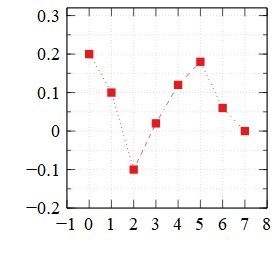
\includegraphics[width=0.32\textwidth]{conv/conv-in}}
    \subfloat[Kernel del filtro]{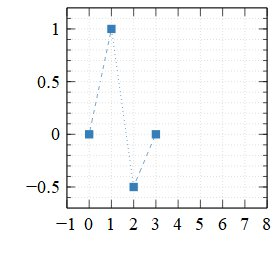
\includegraphics[width=0.32\textwidth]{conv/conv-kr}}
    \subfloat[Risultato]{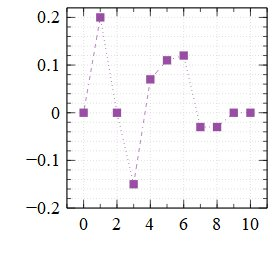
\includegraphics[width=0.32\textwidth]{conv/conv}}
    
    \subfloat[$i=0$]{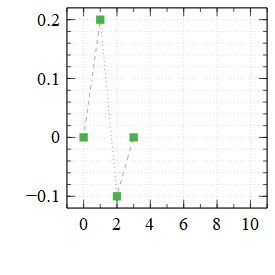
\includegraphics[width=0.25\textwidth]{conv/c1}}
    \subfloat[$i=1$]{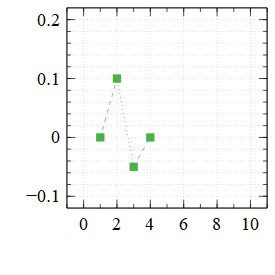
\includegraphics[width=0.25\textwidth]{conv/c2}}
    \subfloat[$i=2$]{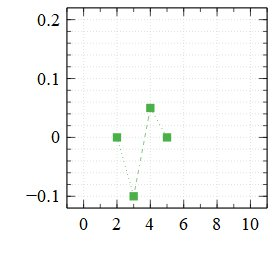
\includegraphics[width=0.25\textwidth]{conv/c3}}
    \subfloat[$i=3$]{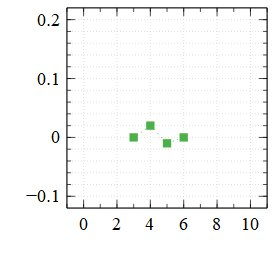
\includegraphics[width=0.25\textwidth]{conv/c4}}
    
    \subfloat[$i=4$]{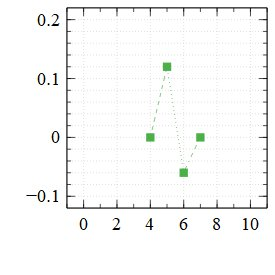
\includegraphics[width=0.25\textwidth]{conv/c5}}
    \subfloat[$i=5$]{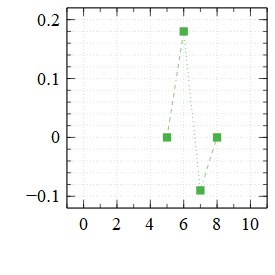
\includegraphics[width=0.25\textwidth]{conv/c6}}
    \subfloat[$i=6$]{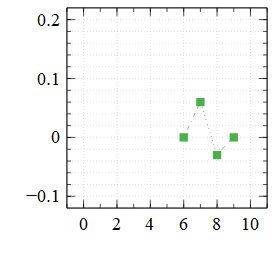
\includegraphics[width=0.25\textwidth]{conv/c7}}
    \subfloat[$i=7$]{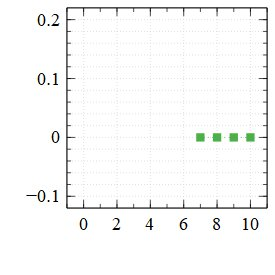
\includegraphics[width=0.25\textwidth]{conv/c8}}
    \caption{Scomposizione dei singoli contributi del segnale in ingresso in una convoluzione.}
    \label{fig:convingresso}
\end{figure}

\begin{comment}
In figura \ref{fig:pulse32conv} si può osservare il risultato della convoluzione di un impulso di 32 campioni con sé stesso ottenuto con l' algoritmo presentato.
\begin{figure}[h]
    \centering
    \subfloat[Impulso]{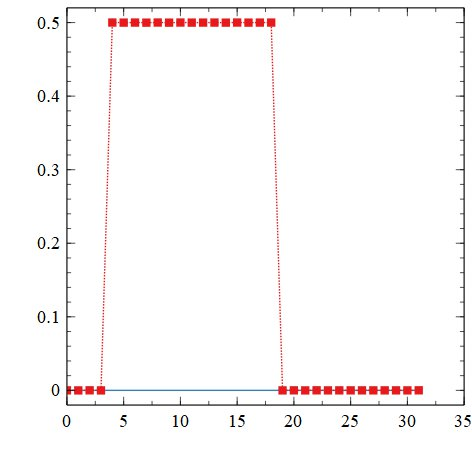
\includegraphics[width=0.5\textwidth]{pulse32}}
    \subfloat[Convoluzione]{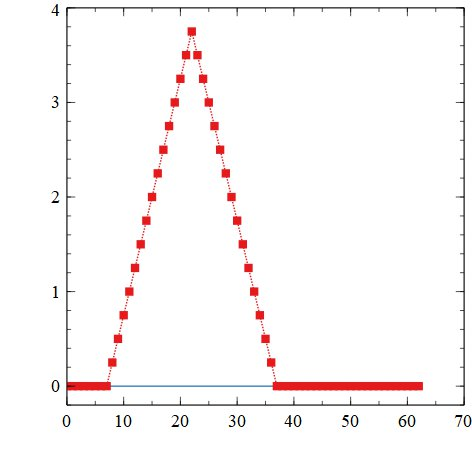
\includegraphics[width=0.5\textwidth]{pulse32conv}}
    \caption{Convoluzione di un impulso rettangolare con sé stesso. In rosso è segnata la parte reale e in blu la parte immaginaria}
    \label{fig:pulse32conv}
\end{figure}
\end{comment}

\subsection{GPU}
Per implementare la convoluzione sulla GPU è necessario individuare i thread che è possibile parallelizzare e racchiuderli in uno o più kernel. Nel caso in esame si è deciso di utilizzare l'implementazione che Smith chiama ``algoritmo dal lato dell'uscita'' \cite[pp.~116-121]{dspguide}, il quale differisce dall'algoritmo precedentemente illustrato nell'implementazione sulla CPU per il fatto che si calcolano i contributi di vari campioni dell'ingresso rispetto ad un solo campione in uscita. I due algoritmi, seppur presentino due punti di vista diversi, sono equivalenti e restituiscono lo stesso risultato.

Bisogna prestare attenzione al fatto che dato un kernel di un filtro di $M$ elementi, il valore dell'elemento $i$-esimo dell'uscita è uguale al prodotto dell'elemento $i-j$ esimo dell'ingresso con l'elemento $j$-esimo del kernel del filtro, con $j = 0 ... M-1$.

Il kernel CUDA utilizzato per compiere questa operazione ridotto alle sue operazioni essenziali è il seguente:

\begin{lstlisting}
__global__ void cudaconvolver_kernel(SignalBuffer_t in_buf, SignalBuffer_t kr_buf, SignalBuffer_t tmp)
{
    int k = blockIdx.x * blockDim.x + threadIdx.x;
    ...
    cuComplex kr_s, in_s;
    cuComplex tmp_s = make_cuComplex(0, 0);
    for (int i = 0; i < kr_buf_size; i++)
    {
        kr_s = get_sample(kr_buf, i);
        in_s = get_sample(in_buf, k-i);
        tmp_s = cuCaddf(tmp_s, cuCmulf(kr_s, in_s));
    }
    set_sample(tmp, index, tmp_s);
    ...
}
\end{lstlisting}

Si noti la presenza dell'indice $k$, il quale viene calcolato in base agli indici del thread corrente e del blocco corrente; esso identifica la posizione $k$ dell'elemento dell'uscita da calcolare. 

Se il segnale in ingresso è composto di $N$ punti e il kernel del filtro è composto da $M$ punti, il segnale in uscita è di $N+M-1$ punti; per questo motivo la funzione kernel viene eseguita $N+M-1$, ovvero è presente una esecuzione della funzione per ogni elemento in uscita.

Nel codice mostrato è stato tolta la parte relativa alla gestione dell'effetto di ``overlap'' in modo da rendere evidenti le parti fondamentali dell' implementazione per la GPU.

È inoltre opportuno specificare che la funzione \lstinline{get_sample} restituisce un numero complesso con parte reale e immaginaria nulla nel caso l'indice richiesto sia all'esterno della dimensione del buffer.

\begin{figure}[h]
    \centering
    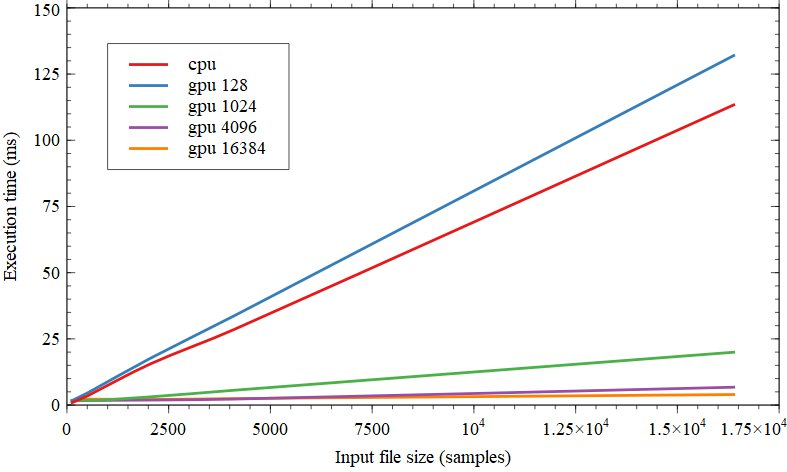
\includegraphics[width=0.85\textwidth]{conv-time}
    \caption{Tempo di convoluzione, CPU e GPU a confronto}
    \label{fig:convtime}
\end{figure}

Il grafico in figura \ref{fig:convtime} rappresenta il tempo necessario per compiere una convoluzione utilizzando un kernel di un filtro di dimensioni fisse (16 punti) al variare della lunghezza del file in ingresso da elaborare. Inoltre per quanto riguarda la GPU sono visualizzati anche valori diversi di lunghezza del buffer di elaborazione, in quanto, a differenza della CPU che non risente della grandezza dello stesso, la GPU presenta prestazioni via via migliori all'aumentare della dimensione del buffer, poiché un buffer più grande significa elaborare più dati in parallelo. Si può anche notare che la GPU ottiene dei tempi di elaborazione peggiori della CPU quando il buffer non è sufficientemente grande: il risultato è giustificato dal fatto che in tale circostanza sono necessari più spostamenti di dati tra memoria RAM e memoria della GPU i quali agiscono da ``collo di bottiglia'' nell'elaborazione. Per come è stato progettato il programma è necessario che un buffer venga elaborato prima che si possa elaborare il seguente (non è possibile elaborare più buffer in parallelo).

\section{DFT}
Un secondo algoritmo interessante da implementare è la trasformata di Fourier discreta. Essa trova larga applicazione come strumento di analisi spettrale dei segnali, oltre ad essere un punto di partenza per poi introdurre la \textit{Fast Fourier Transform} (FFT).

Come indicato nell'equazione \ref{eq:dft}, la DFT è sostanzialmente una sommatoria di un prodotto di numeri complessi, notiamo però che a differenza della equazione della convoluzione (\ref{eq:convoluzionediscreta}) il valore massimo della sommatoria dipende dalla lunghezza del segnale. Questo significa che nella implementazione saranno necessari due cicli \lstinline{for} innestati che dipendono entrambi dalla lunghezza del segnale. Tale configurazione di cicli \lstinline{for} restituisce una complessità computazionale di tipo $O(N^2)$. Motivo ulteriore per cui si è sviluppato l'algoritmo della FFT.

\subsection{CPU}
L'implementazione della trasformata di Fourier discreta è ricavata direttamente dalla sua equazione.

\begin{lstlisting}
void dft(SignalBuffer_t &in_buf, SignalBuffer_t &out_buf, size_t size)
{
    cuComplex s, in_s, out_s;
    ...
    for (size_t k = 0; k < size; k++)
    {
        out_s = get_sample(out_buf, k);
        ...
        for (size_t i = 0; i < size; i++)
        {
            s = cuComplex_exp(-2 * M_PI * k * i / size);
            in_s = get_sample(in_buf, i);
            out_s = cuCaddf(out_s, cuCmulf(s, in_s));
        }
        set_sample(out_buf, k, out_s);
    }
    ...
}
\end{lstlisting}

\lstinline{cuComplex_exp(float x)} è una funzione che restituisce il numero complesso $e^{jx}$. L'algoritmo prende in input un buffer di cui effettuare la trasformata, un buffer in cui inserire il risultato della trasformazione, il canale dei buffer su cui operare e la dimensione in punti della trasformata. Come esposto in precedenza la funzione \lstinline{get_sample} restituisce il numero complesso $0$ nel caso il valore dell'indice sia fuori range. Questo permette di implementare facilmente la DFT di un buffer con un pad di zeri alla sua destra.

\begin{figure}[h]
    \centering
    \subfloat[Impulso]{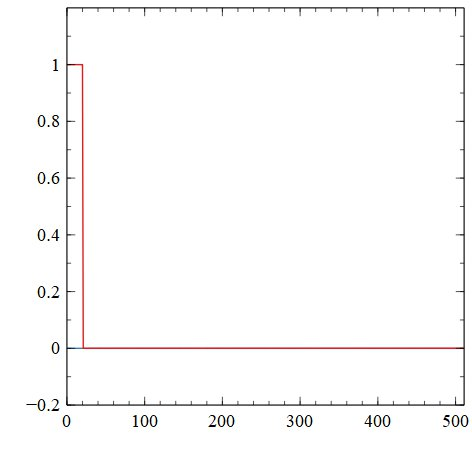
\includegraphics[width=0.4\textwidth]{pulse512}}
    \subfloat[Dft]{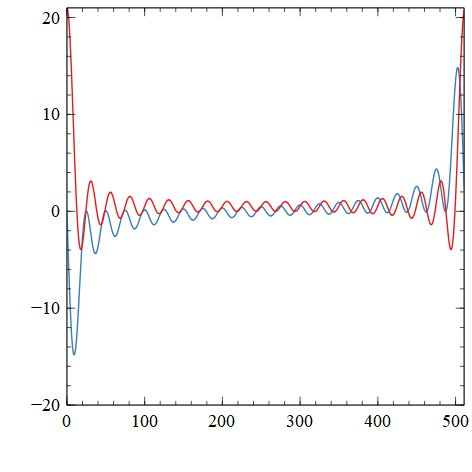
\includegraphics[width=0.4\textwidth]{pulse512dft}}
    \caption{DFT di un impulso di 512 campioni. In rosso è segnata la parte reale e in blu la parte immaginaria}
    \label{fig:pulse512}
\end{figure}

Inserendo nel programma l'impulso di 512 campioni mostrato in figura \ref{fig:pulse512}a si ottiene la trasformata in figura \ref{fig:pulse512}b. Come è facile notare, il segnale di partenza ha solo componente reale, quindi la sua trasformata è simmetrica rispetto a $N/2$ in modo pari per la parte reale e in modo dispari per la parte immaginaria.

\subsection{GPU}
L'operazione di trasformata di Fourier discreta è implementata sulla GPU utilizzando il seguente kernel:

\begin{lstlisting}
__global__ void cudadft_kernel(SignalBuffer_t in_buf, SignalBuffer_t out_buf)
{
    int k = blockIdx.x * blockDim.x + threadIdx.x;
    ...
    size_t size = get_max_buffer_size(out_buf);
    cuComplex out_s = make_cuComplex(0, 0);
    cuComplex in_s, s;
    for (int i = 0; i < size; i++)
    {
        in_s = get_sample(device_buffer, i);
        s = cuComplex_exp(-2.0f * PI * k * i / size);
        out_s = cuCaddf(out_s, cuCmulf(in_s, s));
    }
    set_sample(out_buf, k, out_s);
    ...
}

\end{lstlisting}

Anche in questo caso, il kernel viene eseguito in parallelo su tutti i campioni del segnale risultando più performante della rispettiva implementazione sulla CPU. In particolare si può già notare che la complessità di ogni singolo thread si è ridotta a $O(N)$ e, essendo i thread eseguiti contemporaneamente, la complessità reale non dovrebbe discostarsi troppo da quest'ultima; come dimostrato dai dati relativi al tempo di elaborazione ricavati dal programma e mostrati in figura \ref{fig:dfttime}.

\begin{figure}[h!]
    \centering
    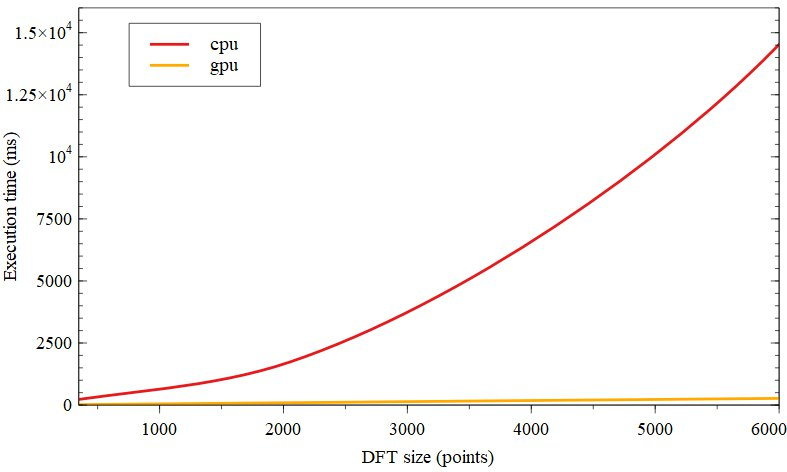
\includegraphics[width=\textwidth]{dft-time}
    \caption{Tempo di calcolo per DFT tra GPU e CPU, al variare del numero di punti della DFT.}
    \label{fig:dfttime}
\end{figure}

\section{Fast Fourier Transform}
L'operazione di DFT è onerosa in termini di calcolo in quanto ha complessità $O(N^2)$, per cui si utilizza spesso la Fast Fourier Transform al suo posto (FFT). Uno degli algoritmi più popolari per il calcolo della FFT è quello ideato da Cooley e Tukey nel 1965. Esso fa uso della decomposizione interlacciata e delle somme a ``farfalla'' le quali permettono all'algoritmo di ottenere una complessità di tipo $O(N log_2N)$ \cite{cooleytukey}.

\subsection{Spiegazione matematica}
La FFT utilizza le proprietà di periodicità e di ``simmetria complessa coniugata'' del numero complesso $e^{-2\pi j\frac{kn}{N}}$ che si può trovare a secondo membro dell'equazione \ref{eq:dft}. Infatti, definendo $W_N=e^{-\frac{2\pi j}{N}}$ è immediato verificare che:

\begin{equation}
    W_N^{k(N-n)} = e^{-2\pi jk}e^{+2\pi j\frac{kn}{N}} = W_N^{-kn} = (W_N^{kn})^\ast
\end{equation}
\begin{equation}
    W_N^{kn} = W_N^{(k+N)n} = W_N^{k(n+N)}
    \label{eq:wnperiodica}
\end{equation}

Separando la sommatoria della DFT in equazione \ref{eq:dft} in termini pari e in termini dispari si ottiene:

\begin{equation}
    X_n = \displaystyle\sum_{k=0}^{N-1}x_k W_N^{kn} = \displaystyle\sum_{k\ pari}x_k W_N^{kn} + \displaystyle\sum_{k\ dispari}x_k W_N^{kn}
\end{equation}

Supponendo $N=2^m$ con $m=\mathbb{N}$, gli indici delle sommatorie possono essere scritti come $2p$ e $2p+1$ con $p=0,1,\dots,\frac{N}{2}-1$:

\begin{equation}
    X_n = \displaystyle\sum_{p=0}^{\frac{N}{2}-1}x_{2p} W_N^{2pn} + \displaystyle\sum_{p=0}^{\frac{N}{2}-1}x_{2p+1} W_N^{(2p+1)n}
\end{equation}

Raccogliendo nella seconda sommatoria si ottiene:

\begin{equation}
    X_n = \displaystyle\sum_{p=0}^{\frac{N}{2}-1}x_{2p} (W_N^2)^{pn} + W_N^{n}\displaystyle\sum_{p=0}^{\frac{N}{2}-1}x_{2p+1} (W_N^2)^{pn}
\end{equation}

Notando che $W_N^2 = e^{-2\pi j\frac{2}{N}} = e^{-\frac{2\pi j}{N/2}} = W_{N/2}$ si ottiene:

\begin{equation}
    X_n = \displaystyle\sum_{p=0}^{\frac{N}{2}-1}x_{2p} W_{N/2}^{pn} + W_N^{n}\displaystyle\sum_{p=0}^{\frac{N}{2}-1}x_{2p+1} W_{N/2}^{pn}
    \label{eq:dftnsu2}
\end{equation}

Le due sommatorie nella \ref{eq:dftnsu2} sono due DFT di ${N/2}$ elementi e la loro somma equivale alla DFT originaria, $X_n$.

Il ragionamento utilizzato fino ad ora si può quindi riapplicare alle DFT di $N/2$ elementi ottenute nella \ref{eq:dftnsu2}, fino ad ottenere, dopo $log_2 N$ volte, delle DFT di un singolo elemento.

Se per una DFT bisogna compiere $N^2$ operazioni, dopo ogni suddivisione in pari/dispari la DFT viene riscritta come due DFT di $N/2$ elementi e $N$ operazioni. Questo significa che il numero di operazioni sono diventate $2(\frac{N}{2})^2 + N = \frac{N^2}{2}+N$ e procedendo in maniera analoga si arriva al numero di operazioni dopo $log_2 N$ suddivisioni: $N + Nlog_2 N$ che equivale, quindi, ad una complessità di $O(Nlog_2 N)$ per $N >> 1$.

\subsection{Spiegazione dell'algoritmo}

\begin{wrapfigure}{r}{0.5\textwidth}
    \centering
    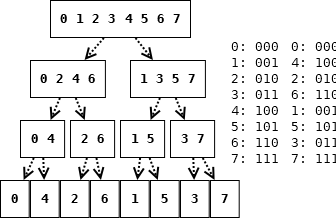
\includegraphics[width=0.40\textwidth]{fft-intrl}
    \caption{Scomposizione interlacciata per il calcolo della FFT di un array di 8 elementi.}
    \label{fig:fftintrl}
\end{wrapfigure}

Data la spiegazione matematica della sezione precedente, è immediato notare che il primo passo per calcolare la FFT di un array di $N=2^m\ ,\ m\in\mathbb{N}$ è quello di riordinare gli elementi in modo che nella prima metà dell'array ci siano gli elementi in posizione pari, mentre nella seconda metà gli elementi di posizione dispari. Dopodiché si ripete questa separazione per i due ``sottoarray'' di $N/2$ elementi. Su un calcolatore ad aritmetica binaria questo è facilmente riconducibile ad un ordinamento a ``bit rovesciati'' degli indici dell'array, come mostrato in figura \ref{fig:fftintrl} per un array di dimensione $N=8$.

In seguito bisogna calcolare la DFT di ogni singolo elemento, un calcolo banale in quanto il risultato della DFT di un singolo elemento è l'elemento stesso.

\begin{wrapfigure}{r}{0.28\textwidth}
    \centering
    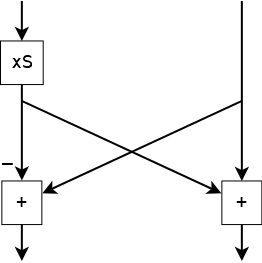
\includegraphics[width=0.20\textwidth]{butterfly}
    \caption{La ``farfalla'', operazione fondamentale per la FFT.}
    \label{fig:fftfarfalla}
\end{wrapfigure}

A questo punto bisogna effettuare le operazioni di somma all'indietro rispettando, quindi, l'ordine con cui si è effettuata la suddivisione dell'array. Notiamo, innanzitutto, che ad ogni ``livello'' di suddivisione si effettua una moltiplicazione e una somma; inoltre è importante notare che in una DFT di $N$ punti si ha $W_N^{k+N/2} = -W_N^k$ e quindi che, grazie alla \ref{eq:wnperiodica}:

\begin{equation}
    X_{n+N/2} = \displaystyle\sum_{p=0}^{\frac{N}{2}-1}x_{2p} W_{N/2}^{pn} - W_N^{n}\displaystyle\sum_{p=0}^{\frac{N}{2}-1}x_{2p+1} W_{N/2}^{pn}
\end{equation}

Disegnando, quindi, un diagramma per il calcolo di $X_n$ e $X_{n+N/2}$ si ottiene un diagramma in figura \ref{fig:fftfarfalla} che viene denominato ``farfalla'' per la sua forma. Le operazioni a ``farfalla'' si combinano dall'array iniziale ordinato a ``bit invertiti'' nel modo raffigurato in figura \ref{fig:fftfarfalle} per un array iniziale di dimensione $N=4$.

\begin{figure}[h]
    \centering
    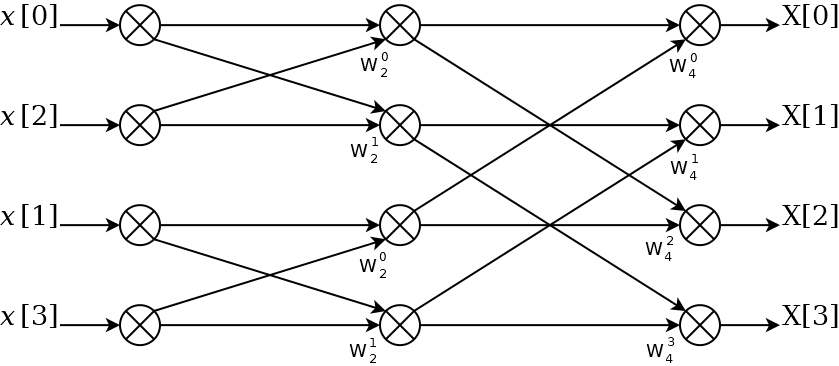
\includegraphics[width=\textwidth]{butterfly-all}
    \caption{Operazioni a farfalla consecutive per il calcolo della FFT di un array di 4 elementi.}
    \label{fig:fftfarfalle}
\end{figure}


\subsection{CPU}
Per implementare sulla CPU la FFT è necessario, quindi, la creazione di una procedura di ordinamento a bit invertiti e una per effettuare le operazioni a ``farfalla''.

\begin{lstlisting}
void fft_wsio(SignalBuffer_t &b_in, SignalBuffer_t &b_out, size_t points)
{
    ... // declare vars, assign sizes
    bit_reversal_sort_wsio(b_in, b_out, points);
    for (size_t level = 0; level < levels; level++){
        ...
        wm = cuComplex_exp(-(M_PI / butterflies_per_dft));
        w = make_cuComplex(1,0);
        for (size_t butterfly = 0; butterfly < butterflies_per_dft; butterfly++){
            for (size_t dft = 0; dft < dfts; dft++){
                ... // calculate indexes
                cuComplex a = get_sample(b_out, index_a);
                cuComplex b = get_sample(b_out, index_b);
                butterfly_calculation(&a, &b, w);
                ... // set out samples
            }
            w = cuCmulf(w, wm);
        }
        ...
    }
}
\end{lstlisting}

Nell'implementazione si può notare che per ogni livello si scorrono prima le operazioni a farfalla e poi le ``sotto DFT'' corrispondenti; in questo modo si può utilizzare lo stesso valore di $W_N^k$ (si faccia riferimento ad esempio alla figura \ref{fig:fftfarfalle}, dove $W_2^0$ e $W_2^1$ appaiono due volte al primo livello). Dopodiché il valore successivo $W_N^{k+1}$ si ricava dalla moltiplicazione di $W_N^k$ con il valore di \lstinline{wm}, il quale contiene il numero complesso con argomento necessario per calcolare $W_N^{k+1}$; questo evita il calcolo tramite funzioni trigonometriche.

\subsection{GPU}

L'implementazione per GPU dell'algoritmo della FFT segue lo stesso schema della CPU, ovvero: si riordina l'array e si effettuano le operazioni a ``farfalla''. La scomposizione in kernel utilizzata consiste nell'operare il riordino tramite una funzione kernel eseguita su ogni elemento dell'array, dopodiché per ogni livello si utilizza un kernel che esegue le somme a farfalla; è chiaro, infatti, che il numero di operazioni a farfalla per ogni livello è uguale a quello degli altri livelli ed è pari ad $N/2$. Quello che cambia da un livello all'altro sono quali coppie di elementi le farfalle elaborano e per questo motivo non è possibile eseguire l'intera FFT con una sola invocazione di kernel, bensì è necessario invocare il kernel per ogni livello (ovvero un numero pari a $log_2 N$ volte), attendendo che i dati siano sincronizzati dopo ogni calcolo.

Il kernel utilizzato per le operazioni a farfalla è qui riportato:

\begin{lstlisting}
__global__ void cudafft_kernel_butterflies(SignalBuffer_t in_buf, SignalBuffer_t out_buf, size_t level)
{
    unsigned int k = blockIdx.x * blockDim.x + threadIdx.x;
    size_t bpd = (size_t)powf(2, level);
    size_t index_a = k + (size_t)(k / bpd) * bpd;
    size_t index_b = index_a + bpd;
    // get a,b samples
    cuComplex w = cuComplex_exp(-(2*PI*index_a)/(bpd*2));
    cuda_butterfly_calculation(&a, &b, w);
    // set a,b samples
}
\end{lstlisting}

La funzione \lstinline{cuda_bufferfly_calculation} esegue l'operazione a farfalla, come nella implementazione per la CPU. La parte interessante del kernel riguarda come ricavare gli indici di \lstinline{a} e \lstinline{b} poiché non è possibile sapere direttamente in quale ``sotto DFT'' è la farfalla, ma è necessario ricavare tale indice.

\begin{figure}[h!]
    \centering
    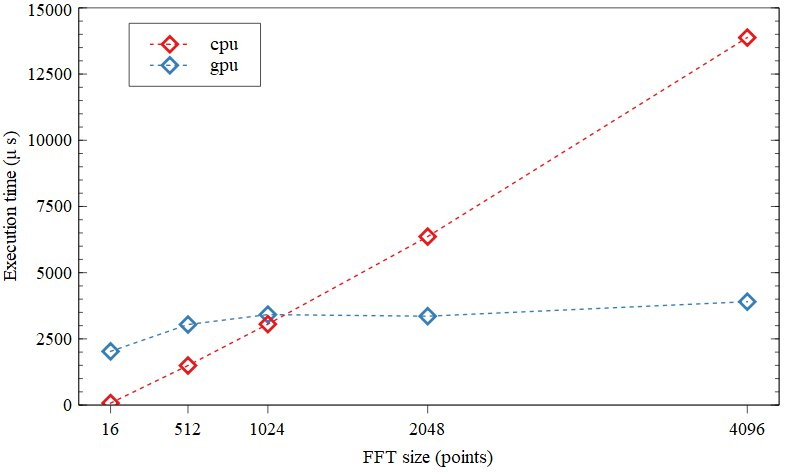
\includegraphics[width=\textwidth]{fft-time}
    \caption{Tempo di calcolo per FFT tra GPU e CPU, al variare del numero di punti della FFT.}
    \label{fig:ffttime}
\end{figure}

In figura \ref{fig:ffttime} sono raffigurati i tempi di calcolo rispetto alla lunghezza della fft. Le linee sono tratteggiate in quanto la FFT non può essere calcolata, con gli algoritmi presentati, per qualsiasi numero di punti, bensì solo per le potenze di $2$. I tempi di elaborazione rispetto alla DFT sono bassissimi (si noti la scala dell'asse $y$ in microsecondi) e la GPU riesce comunque ad ottenere prestazioni migliori al crescere del numero di punti rispetto alla CPU, seppur quest'ultima abbia tempi di calcolo minori per valori di $N$ bassi, dove la GPU non riesce a competere perché è limitata dagli spostamenti di memoria.